\documentclass[border=10pt]{standalone}
\usepackage[T1]{fontenc}
\usepackage{helvet}\renewcommand{\familydefault}{\sfdefault}
\usepackage{tikz}
\usetikzlibrary{positioning,fit,backgrounds,arrows.meta,shapes.geometric,calc}
\definecolor{ink}{HTML}{2A1F18}
\definecolor{inksoft}{HTML}{5C4D40}
\definecolor{terra}{HTML}{B85C38}
\definecolor{moss}{HTML}{4A6B3A}
\definecolor{clay}{HTML}{A9762F}
\definecolor{grey}{HTML}{8B7B6B}
\definecolor{terrafill}{HTML}{FBF1EB}
\definecolor{mossfill}{HTML}{EEF2E8}
\definecolor{clayfill}{HTML}{F7EFDF}
\definecolor{greyfill}{HTML}{F1EDE5}
\begin{document}
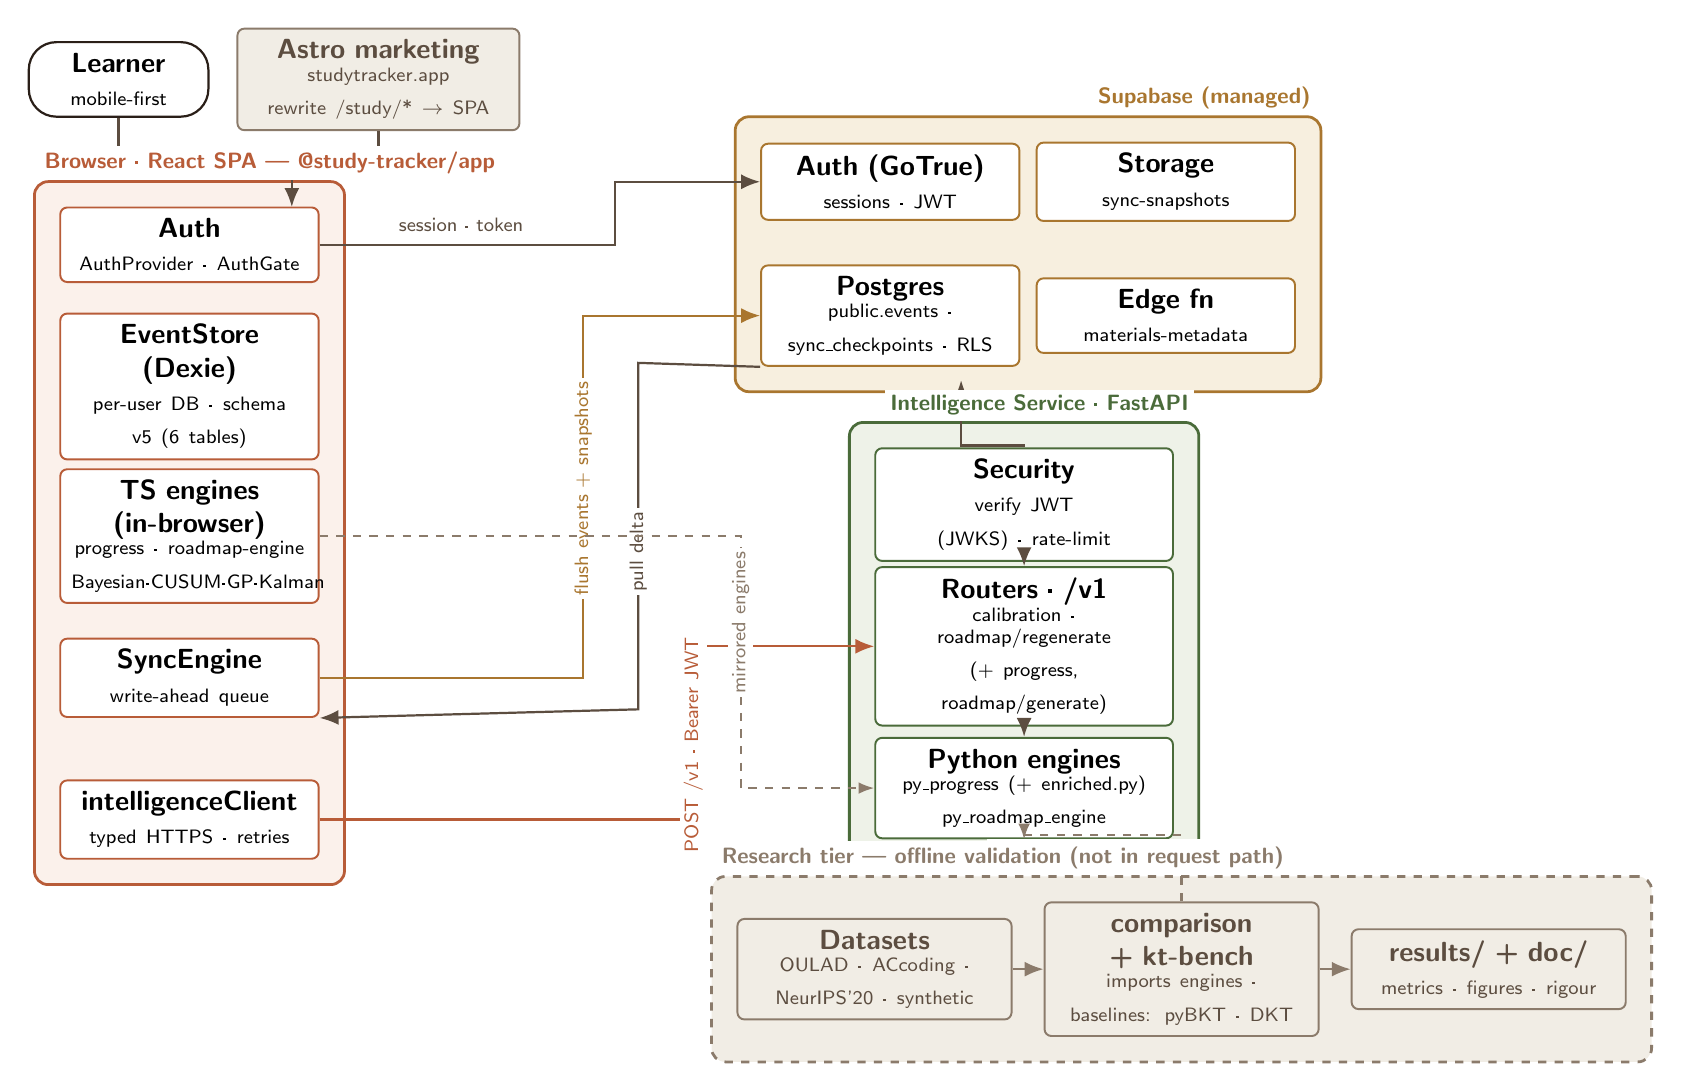
\begin{tikzpicture}[
  font=\sffamily,
  box/.style={rounded corners=2.5pt, draw, line width=0.7pt, align=center, inner sep=4pt, text width=3.0cm, fill=white},
  cli/.style={box, draw=terra},
  dat/.style={box, draw=clay},
  svc/.style={box, draw=moss, text width=3.5cm},
  res/.style={box, draw=grey, fill=greyfill, text=inksoft, text width=3.2cm},
  actor/.style={rounded corners=10pt, draw=ink, line width=0.8pt, align=center, inner sep=4pt, fill=white, text width=2.0cm},
  cont/.style={rounded corners=5pt, line width=1pt, inner sep=9pt},
  ttl/.style={font=\footnotesize\bfseries, fill=white, inner sep=2pt},
  flow/.style={-{Latex[length=2.4mm,width=1.9mm]}, line width=0.8pt, draw=inksoft},
  cflow/.style={flow, draw=terra},
  dflow/.style={flow, draw=clay},
  mirror/.style={-{Latex[length=2mm]}, line width=0.8pt, dashed, draw=grey},
  lbl/.style={font=\scriptsize, fill=white, inner sep=1.3pt, text=inksoft},
  vlbl/.style={lbl, rotate=90},
]

% ---------- actors ----------
\node[actor] (US) at (2.7,12.6) {\textbf{Learner}\\{\scriptsize mobile-first}};
\node[box, text width=3.3cm, draw=grey, fill=greyfill, text=inksoft] (MK) at (6.0,12.6)
  {\textbf{Astro marketing}\\{\scriptsize studytracker.app\\ rewrite /study/* $\to$ SPA}};

% ---------- client column ----------
\node[cli] (CA) at (3.6,10.5) {\textbf{Auth}\\{\scriptsize AuthProvider · AuthGate}};
\node[cli] (CE) at (3.6,8.7)  {\textbf{EventStore (Dexie)}\\{\scriptsize per-user DB · schema v5 (6 tables)}};
\node[cli] (CT) at (3.6,6.8)  {\textbf{TS engines (in-browser)}\\{\scriptsize progress · roadmap-engine\\ Bayesian·CUSUM·GP·Kalman}};
\node[cli] (CS) at (3.6,5.0)  {\textbf{SyncEngine}\\{\scriptsize write-ahead queue}};
\node[cli] (CI) at (3.6,3.2)  {\textbf{intelligenceClient}\\{\scriptsize typed HTTPS · retries}};

% ---------- supabase (right-top) ----------
\node[dat] (SA) at (12.5,11.3) {\textbf{Auth (GoTrue)}\\{\scriptsize sessions · JWT}};
\node[dat] (SS) at (16.0,11.3) {\textbf{Storage}\\{\scriptsize sync-snapshots}};
\node[dat] (SP) at (12.5,9.6)  {\textbf{Postgres}\\{\scriptsize public.events ·\\ sync\_checkpoints · RLS}};
\node[dat] (SE) at (16.0,9.6)  {\textbf{Edge fn}\\{\scriptsize materials-metadata}};

% ---------- intelligence (right-mid) ----------
\node[svc] (IX) at (14.2,7.2) {\textbf{Security}\\{\scriptsize verify JWT (JWKS) · rate-limit}};
\node[svc] (IR) at (14.2,5.4) {\textbf{Routers · /v1}\\{\scriptsize calibration · roadmap/regenerate\\ (+ progress, roadmap/generate)}};
\node[svc] (IP) at (14.2,3.6) {\textbf{Python engines}\\{\scriptsize py\_progress (+ enriched.py)\\ py\_roadmap\_engine}};

% ---------- research (bottom) ----------
\node[res] (RD) at (12.3,1.3) {\textbf{Datasets}\\{\scriptsize OULAD · ACcoding ·\\ NeurIPS'20 · synthetic}};
\node[res] (RC) at (16.2,1.3) {\textbf{comparison + kt-bench}\\{\scriptsize imports engines ·\\ baselines: pyBKT · DKT}};
\node[res] (RR) at (20.1,1.3) {\textbf{results/ + doc/}\\{\scriptsize metrics · figures · rigour}};

% ---------- containers (background) ----------
\begin{scope}[on background layer]
  \node[cont, draw=terra, fill=terrafill, fit=(CA)(CE)(CT)(CS)(CI)] (SPA) {};
  \node[cont, draw=clay,  fill=clayfill, fit=(SA)(SS)(SP)(SE)] (SB) {};
  \node[cont, draw=moss,  fill=mossfill, fit=(IX)(IR)(IP)] (IN) {};
  \node[cont, draw=grey,  dashed, fill=greyfill, fit=(RD)(RC)(RR)] (RS) {};
\end{scope}

% ---------- edges ----------
% learner + marketing into SPA
\draw[flow] (US.south) -- (US.south|-SPA.north);
\draw[flow] (MK.south) -- (6.0,11.5) -- (4.9,11.5) -- (4.9,10.98);

% Auth -> Supabase Auth (top lane)
\draw[flow] (CA.east) -- (9.0,10.5) -- (9.0,11.3) -- (SA.west);
\node[lbl] at (7.05,10.75) {session · token};

% flush events/snapshots  (riser x8.6)
\draw[dflow] (CS.east) -- (8.6,5.0) -- (8.6,9.6) -- (SP.west);
\node[vlbl, text=clay] at (8.6,7.4) {flush events + snapshots};

% pull delta return (riser x9.3)
\draw[flow] (SP.south west) -- (9.3,9.0) -- (9.3,4.6) -- (CS.south east);
\node[vlbl] at (9.3,6.6) {pull delta};

% POST calibration/regenerate (riser x10.0)
\draw[cflow] (CI.east) -- (10.0,3.2) -- (10.0,5.4) -- (IR.west);
\node[vlbl, text=terra] at (10.0,4.15) {POST /v1 · Bearer JWT};

% parity mirror TS <-> Python engines (riser x10.6)
\draw[mirror] (CT.east) -- (10.6,6.8) -- (10.6,3.6) -- (IP.west);
\node[vlbl, text=grey] at (10.6,5.7) {mirrored engines};

% JWKS verify (left side of Intelligence, into Postgres bottom)
\draw[flow] (IX.north) -- (14.2,7.95) -- (13.4,7.95) -- (13.4,8.78);
\node[lbl] at (13.9,8.42) {verify · JWKS};

% internal service arrows
\draw[flow] (IX.south) -- (IR.north);
\draw[flow] (IR.south) -- (IP.north);

% research flow + import
\draw[flow, draw=grey] (RD.east) -- (RC.west);
\draw[flow, draw=grey] (RC.east) -- (RR.west);
\draw[mirror] (RC.north) -- (16.2,3.0) -- (14.2,3.0) -- (IP.south);
\node[lbl, text=grey] at (15.1,2.78) {imports engines (offline)};

% ---------- container titles (top, opaque) ----------
\node[ttl, text=terra, anchor=south west] at ([xshift=2pt]SPA.north west) {Browser · React SPA — @study-tracker/app};
\node[ttl, text=clay,  anchor=south east] at ([xshift=-2pt]SB.north east) {Supabase (managed)};
\node[ttl, text=moss,  anchor=south east] at ([xshift=-2pt]IN.north east) {Intelligence Service · FastAPI};
\node[ttl, text=grey,  anchor=south west] at ([xshift=2pt]RS.north west) {Research tier — offline validation (not in request path)};

\end{tikzpicture}
\end{document}
